\section{Current problems}

Using the information system of NTNU on a daily basis provided us with the knowledge of few weaknesses. In order to try and improve it we gathered some problems that occurred to us so that we will be able to get rid of those once we build the structure of the new system. Here are the main problems we have seen:
\begin{itemize}

\item{All the systems (i.e. innsida, studentweb, itslearning) are separate, making information more difficult to access, too spread.}
\item{Studentweb generates new links every time you go to a new site.}
\item{Masterstudents use a different page, the system in whole is unintuitive since you also need information from other systems.}
\item{Impossible to check your grades for assignment and exam on the same page. If the assignments count towards your final grade you have to make an extra step to find the grade you have just got.}
\item{Need to login separately on every site, even though it is the same FEIDE-login.}
\item{Some redundancies, figure {\ref{fig:redundancy}} is an example.}
\item{The daily update must occur if you changed anything that needs communication between systems, otherwise it won't be displayed}
\item{Many of the systems have fields and services that are almost not used or simply unnecessary, like calendar on It's learning, emails on Student web or course table on Innsida. }
\end{itemize}

\begin{figure}[H]
	\begin{center}
		\centerline{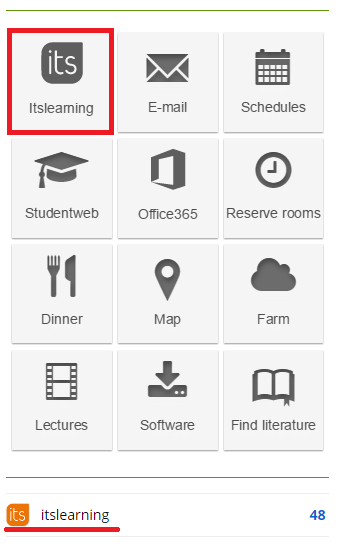
\includegraphics[scale=0.6]{redundancy}}
		\caption[Redundancy in innsida]{Redundancy in innsida}
		\label{fig:redundancy}
	\end{center}
\end{figure}

Using the current system, a BPMN model has been made through the process of registering for a course and exam, an check afterwards whether the user has been accepted to the course or not. See figure  {\ref{fig:addcourse}}.
\par
The actors involved in this process are the user, Studentweb and Itslearning. That's two different systems for one process that is only about one course. The tasks that the user has to accomplish are easy and not annoying so far, this side of the process is quite good. Only two databases are updated, that is also fine. The issue is one listed above, Since the user has to register on Studentweb and check on Itslearning, a communication has to be done between them. The fact is a maintenance occurs daily, and from that, all the information is updated.
\par
As a result, to check any information on the course you just added, you have to wait the daily maintenance other you won't be able to see if you are even accepted to this course.

\begin{figure}[H]
	\begin{center}
		\centerline{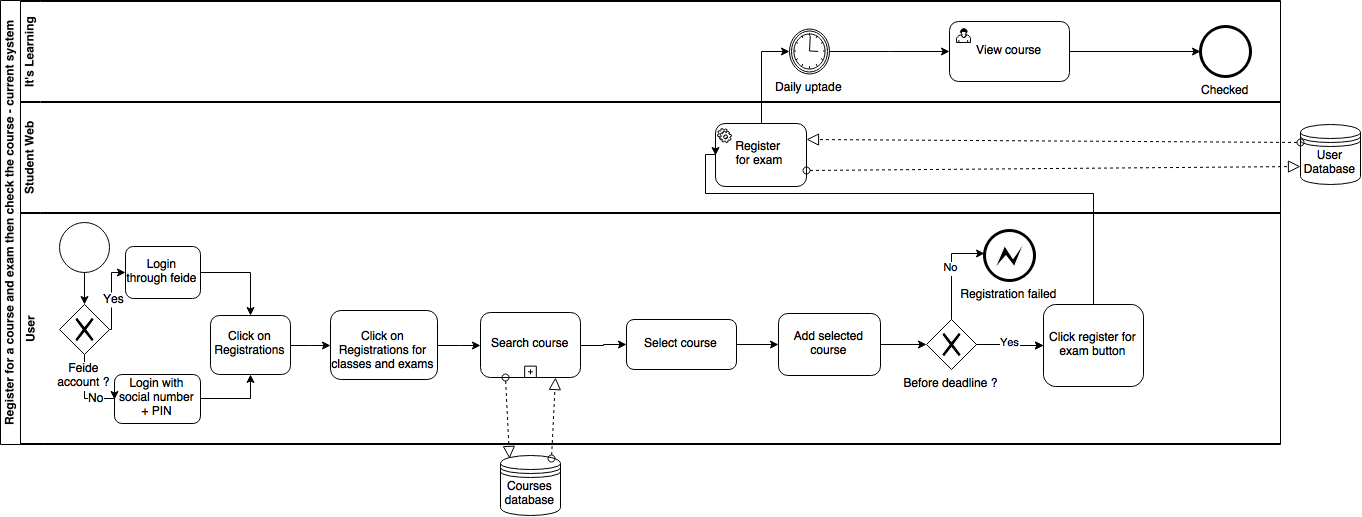
\includegraphics[scale=0.4]{addcoursecurrentsystem}}
		\caption[Register for a course and exam then check - current system]{Register for a course and exam then check - current system}
		\label{fig:addcourse}
	\end{center}
\end{figure}

This matter will be discussed in the next part, a BPMN model will show how it will be in the new system. Also, some other improvements will be stated through BPMN models such as a new way to send e-mails and to complain about a grade. 
